\documentclass[12pt, a4paper]{article}
\RequirePackage[hmargin=2cm,vmargin=2cm]{geometry}

\usepackage[T1]{fontenc}
\usepackage{lmodern}
\usepackage{amssymb,amsmath}
\usepackage{authblk} % allows for better author affiliations

%appendix
\usepackage[title,titletoc,toc]{appendix}
\usepackage{setspace}  % for double spacing

% Fancy HEADER
\usepackage{fancyhdr}
\pagestyle{fancy}
\setlength{\headheight}{15pt}
\pagenumbering{arabic}
\lhead{\itshape{\nouppercase{\leftmark}}}
\chead{}
\rhead{\thepage}
%\lfoot{v }
\cfoot{}
%\rfoot{\thepage}

% allows for numbered referencing, as required by ecol letters
\usepackage{etoolbox}
\newbool{MyRefNumbers}
\booltrue{MyRefNumbers} % comment to remove numbers in reference list

\usepackage{natbib}
\bibliographystyle{ecol_let}
\setcitestyle{authoryear,open={(},close={)}}

\usepackage{graphicx}
\graphicspath{{../output/}}

% We will generate all images so they have a width \maxwidth. This means
% that they will get their normal width if they fit onto the page, but
% are scaled down if they would overflow the margins.
\makeatletter
\def\maxwidth{\ifdim\Gin@nat@width>\linewidth\linewidth
\else\Gin@nat@width\fi}
\makeatother

\let\Oldincludegraphics\includegraphics
\renewcommand{\includegraphics}[1]{\Oldincludegraphics[width=\maxwidth]{#1}}

\usepackage[rgb,dvipsnames]{xcolor}
\definecolor{grey}{rgb}{0.5, 0.5, 0.5}

\usepackage[setpagesize=false, % page size defined by xetex
              unicode=false, % unicode breaks when used with xetex
              xetex]{hyperref}
\hypersetup{breaklinks=true,
            pdfauthor={},
            pdftitle={Untangling the link between traits, size and growth rate in plants},
            colorlinks=true,
            citecolor=black,
            urlcolor=grey,
            linkcolor=grey}
\setlength{\parindent}{0pt}
\setlength{\parskip}{6pt plus 2pt minus 1pt}
\setlength{\emergencystretch}{3em}  % prevent overfull lines

\title{\LARGE Untangling the link between traits, size and growth rate in plants}

\author[1]{Daniel S. Falster}
\author[1]{Richard G. FitzJohn}

\affil[1]{{\footnotesize Biological Sciences, Macquarie University, North Ryde, NSW 2109, Australia}}
\renewcommand\Authands{ and }
\date{\vspace{-3em}}

\begin{document}

\maketitle
\thispagestyle{empty} % avoid header and footer on first page. Put after \maketitile, if using that

\section{Ideas}\label{abstract}

Table near intro summarising empricial patterns to be explained by integrated model?

Section 3.3 of King (2005) shows that the cost of turning over leaves, branches and fine roots may halve the height growth rate that could otherwise be attained.

King 1999 also predicts a change in the SLA optimising growth rate, via a cross correlation with self shading. Basically, the much greater path length from roots to leaves in trees vs. seedlings results in a much greater increment in support cost per increment in crown area for trees. This explanation is treated by the growth model of King (1999), which predicts that the SLA maximizing growth rate declines as seedlings grow larger, even before the onset of leaf turnover.

\section{Abstract}\label{abstract}

\section{Introduction}\label{introduction}

Functional traits capture core differences in the strategies
plants use to generate and invest surplus energy
 \citep{Wright-2004, Chave-2009, Westoby-2002}.
Although most plants have the same basic physiological function
and key resource requirements (carbon, nitrogen and water), species differ considerably in
rates at which resources are acquired and invested into different tissues.
Much of this functional variation relates to underlying
differences in some prominent traits, including leaf
mass per area (LMA), wood density (WD), leaf nitrogen per area, vessel
diameter,  maximum  height (HMAX) and seed size  \citep{Wright-2004, Chave-2009}.
Data for these traits now exists for up to 10\% of the world's 250000 plant species
\citep{Cornwell-2014}. Increasingly, researchers have been looking to traits
as potential indicators of the growth strategy and ecology of a species.

While the influence of plant traits on elements of plant physiological
function is increasingly understood, attempts at using traits to understand
demographic rates have met with mixed success
 \citep{Wright-2010, Poorter-2008}. In seedlings, the trait LMA
-- the central element of the leaf economics spectrum
 \citep{Wright-2004} -- has been tightly related to relative growth
rate in plant mass \citep{Lambers-1992, Wright-2000}. LMA and
its correlate leaf lifespan have also been linked to height growth rate for
small seedlings and saplings \citep{Reich-1992, Poorter-2006}. These
early successes prompted researchers to search for similar relationships in
large plants. However, the results showed that in trees LMA was not correlated
with diameter growth rate  \citep{Wright-2010, Poorter-2008,
Herault-2011}. Meanwhile, other traits such as wood density showed
strong relationships to growth in large plants \citep{Wright-2010},
but only weak relationships in seedlings  \citep{Castro-1998}. Thus
far, most trait growth relationships have been quantified for one or few
traits and at a single life- stage. Yet the picture is emerging is that the
link between traits and growth may be modified by plant size
 \citep{Ruger-2012}. This finding challenges a wide-spread
assumption regarding traits: that particular ends of the trait spectrum translate directly into
faster or slower growth (refs XX).

The challenge of interpreting diverse empirical results seeking to link
traits to growth rate is made all the harder because we currently lack clear
expectations on the expected signal. Generating such expectations is one of the
primary role for theory \citep{Kokko-2007}. Current empirical
results suggest the effect of traits on growth changes with size and possibly
also light environment, yet current theory says little about how such
relationships might come about. A widely-used model shows that for seedlings,
mass-based relative growth rate is linearly and negatively related to LMA
 \citep{Lambers-1992, Cornelissen-1996, Wright-2000}.
 An extension of the model suggests a similar
relationship may hold at larger sizes \citep{Enquist-2007}. But as
described above, this prediction is not supported by empirical results.
Meanwhile, theoretical predictions on how other traits should influence growth
are largely absent.

A further problem with existing theory is that the effects of traits are all
realised via influences on mass production \citep{Enquist-2007},
whereas the effect of traits such as LMA, WD, and Hmax is via allocated
to different tissues \citep{Falster-2011}. There are in fact two problems with theory
focussed solely on mass production. The first is that measuring mass
production is only practical for small plants that can be easily harvested.
For larger plants, growth is more often measured as increment in either diameter
or height. For example, the CTFS monitors diameter growth in 49 large permanent
plots across forests worldwide \citep{Anderson-2015};
 forestry have likewise recorded growth in diameter across
large tracts of the globe \citep{Purves-2008}. The second problem is
that, as we outline further below, because mass production is only one
component of plant growth; theory focussing solely on mass production will
 always be limited.

Effect of traits on shade tolerance also porrly udnerstood. Empirical -- shade

(reich 1992, Niinements 2010, Gower-1993 - both show higher LAI in high LMA / long LL stands)

Ultimately, trait based understanding integrated wiht model of plant growth, also able to cpature patterns of growth through ontogeny. Growth rates tend to show hump-shaped relationship with size, when expressed as either height \citep{Sillett-2010, King-2011} or diameter growth \citep{Herault-2011}.  In contrast, basal-area growth continues to increase with size \citep{Sillett-2010, Stephenson-2014}, due to an increasing influence of stem turnover. All growth measures decrease sharply with size when expressed as relative growth rates \citep{Rees-2010, Iida-2014}. Shade tolerance tends to decrease with increasing size \citep{Lusk-2006}, due to increasing costs of mainatining stems \citep{Givnish-1988}

In this paper we provide a mechanistic framework for describing the potential
effect of traits on growth throughout a plant's life-cycle, linking to
commonly used metrics such as height and diameter growth. To help motivate our
study we re-analyse demographic and trait data from an earlier study
 \citep{Wright-2010}, to show 1) that the link between traits and
growth is stronger than previously thought, 2) that the influence of three
prominent traits on growth rate is moderated by plant size, and 3) that the
impact of size on the nature of relationships varies among traits
 \citep[see also]{Ruger-2012}. We then show how these results align with new
set of theoretical predictions. Analysis extends ...
Moreover, we show how traits moderate plant
responses to light environment and also determine shade tolerance, supporting
diverse empirical results \citep{Ruger-2012, Poorter-2006}. By
disentangling the effects of plant size, light environment and traits on
growth rates, we hope to provide a solid theoretical foundation for trait
ecology and thus provide a platform for understanding growth across diverse
species around the world.

\section{Materials and Methods}\label{materials-and-methods}

\subsection{Growth data}\label{growth-data}


\subsection{Conceptual framework}\label{conceptual-framework}

To make sense of empirical patterns, we extend a widely-used theoretical model that links growth rate in
seedlings to LMA \citep{Lambers-1992, Wright-2000}, to explicitly include influences of
size, light environment, and other prominent traits. This model

Builds on 2011 paper - highlight what's new from there.

First derive ... generally true.

Eqs. \ref{eq:dhdt}-\ref{eq:dDdt} are mathematically true, and must
therefore hold for any model of plant growth. To make explicit
predictions, however, requires two additional elements: 1) A specific
model describing how the various mass and area terms
($M_{\rm l}, M_\textrm{s}, M_{\rm b}, M_{\rm r}, A_{\rm l}, A_\textrm{s}, A_{\rm b}$)
vary relative to one another; and 2) For any trade-offs in plant
function to be specified; this is where traits have an influence.  These two components are outlined in following sections.

\subsubsection{Standard model for mass production}

We begin with a standard model for the amount of biomass available for
growth, ${\rm d}B / {\rm d}t$, given by the difference between income
(total photosynthesis) and losses (respiration and turnover) within the
plant \citep{Makela-1997, Thornley-2000, Falster-2011}:

\begin{equation}\label{eq:dbdt}
\underbrace{\strut \frac{{\rm d}B}{{\rm d}t}}_\textrm{net biomass production}
  = \underbrace{\strut y}_\textrm{yield}
    \big( \underbrace{\strut A_{\rm l} \, p}_\textrm{photosynthesis} -
     \underbrace{\strut \,\sum_\textrm{i=l,b,s,r}{M_\textrm{i} \, r_\textrm{i}}}_\textrm{respiration}\big)
    - \underbrace{\strut \sum_\textrm{i=l,b,s,r}{M_\textrm{i} \, k_\textrm{i}}}_\textrm{turnover}.
\end{equation}

Here, $m,r$, and $k$ refer to the mass, respiration rate, and
turnover rate of different tissues, denoted by subscripts $l$=leaves,
$b$=bark, $s$=sapwood and $r$=roots. $A$ is the assimilation
rate of CO$_2$ per leaf area and $y$ is yield: the fraction of
assimilated carbon fixed in biomass (the remaining fraction being lost
as growth respiration) (see Table \ref{tab:params} for units and
definitions). Photosynthesis is proportional to leaf area,
$A_{\rm l} = M_{\rm l} / \phi$, where $\phi$ is leaf mass per area.
The total mass of living tissues $M_{\rm a}=M_{\rm l}+M_{\rm b}+M_\textrm{s}+M_{\rm r}.$

The only potentially controversial element of in eq. \ref{eq:dbdt} is that it assumes tissues lost via turnover are replaced before energy is allocation to either new growth or reproduction \citep{Thornley-2000}. This assumption is likely to hold true for most woody plants, because the ..... However, the assumption may not hold for some herbs or annuals, where the swicth to reproduction often entails run-down in the vegtative part of the plant (refs XX) \citep{ Thornley-2000}.

\subsubsection{Decomposing height, basal area and diameter growth}

To model growth in either height, basal area or stem diameter requires that account not just for mass production, but also for the costs of building new tissues, allocation to reproduction, and architectural layout. Mathematically, height growth can be decomposed into a product of physiologically relevant terms \citep{Falster-2011}:

\begin{equation} \label{eq:dhdt}
\underbrace{\strut\frac{{\rm d}H}{{\rm d}t}}_\textrm{height growth rate}= \underbrace{\strut\frac{{\rm d}H}{{\rm d}A_{\rm l}}}_\textrm{architecture}
\times \underbrace{\strut\frac{{\rm d}A_{\rm l}}{{\rm d}M_{\rm a}}}_\textrm{marginal leaf deployment}
\times \underbrace{\strut\frac{{\rm d}M_{\rm a}}{{\rm d}B}}_\textrm{allocation to growth}
\times \underbrace{\strut\frac{{\rm d}B}{{\rm d}t}}_\textrm{mass production}.
\end{equation}

The first term on the right of eq \ref{eq:dhdt},
${\rm d}H / {\rm d}A_{\rm l}$, is the growth in plant height
per unit growth in total leaf area -- accounting for the architectural
strategy of the plant. Some species tend to leaf out more than grow
tall, while other species emphasise vertical
extension \citep{Poorter-2006}.

The second term, ${\rm d}A_{\rm l} / {\rm d}M_{\rm a}$,
accounts for the marginal cost of deploying an additional unit of leaf
area, including construction of the leaf itself and various support
structures. As such, ${\rm d}A_{\rm l} / {\rm d}M_{\rm a}$
can itself be expressed as a sum of construction costs per unit leaf
area:

\begin{equation}\label{eq:daldmt}
\frac{{\rm d}A_{\rm l}}{{\rm d}M_{\rm a}}
= \big(\phi
 + \frac{{\rm d}M_\textrm{s}}{{\rm d}A_{\rm l}} + \frac{{\rm d}M_{\rm b}}{{\rm d}A_{\rm l}} + \frac{{\rm d}M_{\rm r}}{{\rm d}A_{\rm l}}\big)^{-1}.
\end{equation}

The third term in eq \ref{eq:dhdt},
${\rm d}M_{\rm a} / {\rm d}P$, gives the fraction of net
biomass production (eq. \ref{eq:dbdt}) that is allocated to growth
rather than reproduction or storage.

In a similar way, basal area ($A_{\rm st}$) increment can be
expressed as the sum of increments in sapwood, bark \& heartwood areas
($A_\textrm{ss}, A_{\rm sb}, A_{\rm sh}$ respectively):
$\frac{{\rm d}A_{\rm st}}{{\rm d}t}= \frac{{\rm d}A_{\rm sb}}{{\rm d}t} + \frac{{\rm d}A_\textrm{ss}}{{\rm d}t} + \frac{{\rm d}A_{\rm sh}}{{\rm d}t}$.
We now have an equation for basal area growth that conatins many of the same
elements as eq. \ref{eq:dhdt}:

\begin{equation}\label{eq:dast}
\frac{{\rm d}A_{\rm st}}{{\rm d}t}=
\left(\frac{{\rm d}A_\textrm{ss}}{{\rm d}A_{\rm l}} + \frac{{\rm d}A_{\rm sb}}{{\rm d}A_{\rm l}}\right) \times
\frac{{\rm d}A_{\rm l}}{{\rm d}M_{\rm a}} \times \frac{{\rm d}M_{\rm a}}{{\rm d}B} \times \frac{{\rm d}B}{{\rm d}t} +\frac{{\rm d}A_{\rm sh}}{{\rm d}t} .
\end{equation}

Diameter growth is then given by the geometric relationship between stem
diameter ($D$) and $A_{\rm st}$:

\begin{equation} \label{eq:dDdt}
\frac{{\rm d}D}{{\rm d}t}= \sqrt{\frac{\pi}{A_{\rm st}}} \frac{{\rm d}A_{\rm st}}{{\rm d}t}.
\end{equation}

\subsubsection{A functional-balance model for allocation}

To address the first of these challenges, we use a functional balance
model \citep{Yokozawa-1995, Falster-2011} assuming
1) an allometric relation between total leaf area and plant height, and
2) a constant ratio between total leaf area and each of sapwood
cross-sectional area, bark cross-sectional area, and total root mass.
These assumptions, which are well-supported by data (Fig.
\ref{f-assumptions}), lead immediately to an allometric model for plant
size (Table \ref{tab:allometry}, see Supplementary material for
derivations). Substituting from Table \ref{tab:allometry} into eqs.
\ref{eq:dhdt}, \ref{eq:dast}, \ref{eq:dDdt} then gives an explicit model
for plant growth in relation to size.


\begin{itemize}
\itemsep1pt\parskip0pt\parsep0pt
\item
  four key assumptions.
\item
  simple linear functions non-critical for results of this paper,
\item
  explore using an example model, but any model with basic size effects
  will display same behaviour

  \begin{itemize}
  \itemsep1pt\parskip0pt\parsep0pt
  \item
    details about our model ()
  \item
    show argument hold intuitively
  \end{itemize}
\end{itemize}

\subsubsection{Embeeding trait-related trade-offs}

use table with arrows to



By definition, the main effect of increasing $\phi$ is to decrease the
marginal leaf deployment per mass (eq. \ref{eq:daldmt}) and thus reduce
growth rate. However, to fully account for the influence of $\phi$ on
growth we must also account for the decrease in leaf turnover that
results from superior leaf construction \citep{Wright-2004}.
This is achieved by linking the turnover rate of leaf in eq.
\ref{eq:dbdt} to $\phi$. We use an allometric scaling relationship of
the form $k_{\rm l}=\alpha_4 \, \phi^{-\beta_4}$, which has been
shown to describe patterns across diverse
ecosystems \citep{Wright-2004} (Fig. \ref{fS-leaf}).

As for leaf, cheaper stem construction (lower $\rho$) decreases the
cost of deploying a unit of leaf area, and may thereby increase growth
rates. However, the cost of cheap stem construction must also be
accounted for. However, the direct physiological trade-offs of lower
$\rho$ are less understood than for $\phi$. One possibility is that
lower $\rho$ decreases mechanical strength resulting in higher
mortality \citep{Chave-2009, Wright-2010}. Under
this scenario, decreasing $\rho$ will always provide a growth
advantage, because the costs of low $\rho$ are not realised within the
terms of eqs. \ref{eq:dhdt} and \ref{eq:dast} (Table
\ref{tab:trade-offs}). In addition, lower $\rho$ may increase turnover
of sapwood. Mirroring our assumptions for leaves, we let sapwood
turnover decrease with $\rho$,
i.e.$k_\textrm{ss}=\alpha_5 \, \rho^{-\beta_5}$, with $\beta_5 > 1$.

Unlike leaf and stem traits, height at maturation ($h_m$) moderates
growth by adjusting the amount of energy invested in growth, i.e.~the
term $\frac{{\rm d}M_{\rm a}}{{\rm d}B}$ in eqs.
\ref{eq:dhdt} and \ref{eq:dast}.

\subsection{Analysis}\label{analysis}



\newpage
\section{Results and Discussion}\label{results}

\subsection{Changes in growth rate with size}

This new growth model captures the intrinsically size-dependent nature
of plant growth, recovering well-known
empirical patterns \citep{Sillett-2010, King-2011}. Height growth shows a hump-shaped pattern
with size, first increasing then decreasing. This pattern results from
systematic changes in the four components of eq. \ref{eq:dhdt} with size
(Fig. \ref{f-conceptual}), including a strong decline in the fraction of plant
that is leaf declines with increasing size (Fig. \ref{f-mass_fraction}),
and increasing reproductive allocation. In contrast, basal-area growth
continues to increase with size \citep{Sillett-2010, Stephenson-2014},
due to an increasing influence of stem
turnover. Diameter growth shows a weakly hump shaped
curve \citep{Herault-2011}, tapering off slightly at larger
sizes, in part because of allometric effects (eq. \ref{eq:dDdt}, but
mainly because of increased reproductive allocation in older trees
(Fig?). All growth measures decrease sharply with size when expressed as
relative growth rates \citep{Iida-2014}.


\subsection{How traits influence growth rate}

\subsubsection{LMA}

Unlike eq. \ref{eq:RGR}, eqs. \ref{eq:dhdt}, \ref{eq:dast} and
\ref{eq:dDdt} predict a relationship between $\phi$ and growth that
changes with plant size ( \ref{f-lmA_growth_size}).
Decreasing $\phi$ has two impacts on growth rate. First, lower
$\phi$ increases marginal leaf deployment
(${\rm d}A_{\rm l} / {\rm d}M_{\rm a}$ by economising on
construction costs. Second, lower $\phi$ decreases net production
(${\rm d}P / {\rm d}t$), due to increased leaf turnover. Whether
lower $\phi$ increases growth thus depends on the relative magnitude
of these two effects. When plants are small the effect on leaf
deployment rate is bigger and so decreasing $\phi$ increases growth
rate. When plants are large, the influence of $\phi$ on leaf
deployment rate is diminished, because the costs of building other
supportive tissues (other terms in eq. \ref{eq:daldmt}) are larger (Fig.
\ref{f-mass_fraction}). The net result is that at larger sizes, low
$\phi$ is no longer advantageous for growth (Fig.
\ref{f-lmA_growth_size}d).

\subsubsection{Wood density}

Under this scenario, decreasing $\rho$ provides an advantage in height
growth only when the benefits of low $\rho$ outweigh the costs. This
effect is strongest at intermediate sizes. The decline in height growth
at low $\rho$ with size is more marked than for either stem basal-area
and diameter growth, because high sapwood turnover also contributes to
this growth measure. Thus diameter growth continues, even as net
production approaches zero.

\subsubsection{hmat}

 Greater height at maturation ($h_m$)
can thus lead to a growth advantage by increasing
$\frac{{\rm d}M_{\rm a}}{{\rm d}B}$ . At smaller sizes, there is no differentiation
among species, because most species are focusing on growth. At larger sizes, individuals of some species are
allocating a majority of their surplus energy to growth, leaving a
strong signal in potential growth rate.


\subsubsection{Responsiveness to light}

Two other important predictions arise directly from linking traits to
growth rate. First, traits moderate the
responsiveness of growth to changes in light environment. This response
arises simply because species with higher potential growth rate have
greater potential plasticity. Recent analyses have shown that species
with low $rho$ increase growth more substantially with incraeses in
light \citep{Ruger-2012}. This is exactly the behaviour
exhibited in our model (Fig. \ref{f-growth_light_dia}), at least for small
to intermediate sizes. At larger sizes (D=0.2m) however, the advantages
of low $\phi$ are lost (Fig. \ref{f-growth_light_dia}). This results also
agrees with empirical results showing that growth for species with low
$rho$ actually decreases as size
increases \citep{Ruger-2012}. In contrast, growth rate tends
to increase in size for the species with highest
$\rho$ \citep{Ruger-2012}.


Variation in $\phi$ also moderates the response of growth to changes
in light, with species having the lowest $rho$ being most responsive.
However, unlike for $\rho$, the effect appears only for the smallest
size classes. Accordingly, empirical analyses have detected such a link
in small plants but not for plants \textgreater{} 0.01m
dbh \citep{Ruger-2012}.

\subsection{Growth is more than just photosynthesis}\label{tree-growth-is-more-than-just-photosynthesis}

Current theory emphasises the relationship between $\phi$ and the relative growth in plant mass
\citep{Lambers-1992, Cornelissen-1996, Wright-2000, Enquist-2007},
${\rm d}P / {\rm d}t / M_{\rm a}$. This relationship can be derived from eq. \ref{eq:dbdt}  by ...
(see Appendix \ref{app:traits-RGR}).

Recently realisation that allocation and turnover major areas of
uncertainty

Model reconciles idea that traits can have negative impact on carbon
budget, but still have positive influence on growth rates

\begin{itemize}
\itemsep1pt\parskip0pt\parsep0pt
\item
  Enquist 2007: sla and wd increase mass-production, where as in our
  theory effects on mass production are negative. (also contradicts
  earlier model from Enquist 1999, where argued wood density had no
  effect on mass production)
\end{itemize}

Assumes low lma and wd used to reduce costs of building leaf and stem,
ie. total leaf area and stem corss section remains same. In this way
differs to assumptions of recent work by anten\_role\_2010,
larjavaara\_rethinking\_2010.

Model is realisation of several ideas that have been around for some
time.

Plasticity in trait values predicted from model:

@Osazuwa-2014 - indreases in WD through ontogeny.

\subsection{Shade tolerance}\label{shade-tolerance}

Second, species with low $\phi$ and low $\rho$ are predicted to be
less shade tolerant (Fig. \ref{f-wplcp}). At low $\phi$ ($\rho$),
leaf (sapwood) turnover is higher and thus a greater light income is
needed to offset these costs. As previously suggested
 \citep{Givnish-1988}, shade-tolerance also decreases with
height because as size increase, the total amount of energy needed to
offset respiratory and turnover costs in the stem also increases. These
finding matches well known empirical patterns, where both $\phi$ and
$\rho$ have been linked to shade tolerance \citep{Poorter-2006, Lusk-2008,osunkoya-1996}.

Results fo poort \& binger for surival strongest for LL.

Also baltzer.

\subsection{Implications for trait-based approaches}\label{implications-for-trait-based-approaches}

How do comparative people interpret sla now - beyond fast slow.

Think about traits as defining potential trajectory, rather than making
species fast or slow growing per se.

Selection on traits in different parts of lifecycle

Trait plasticity - can explain, no clear advantage of low lma at large
sizes

Framework for generalising about effect of traits


Towards a global model of growth:

\begin{itemize}
\itemsep1pt\parskip0pt\parsep0pt
\item
  mechanistic model of height and dbh growth which accounts for effects
  of size, light environment and traits

  \begin{itemize}
  \itemsep1pt\parskip0pt\parsep0pt
  \item
    need to account for size long recognized, but not straightforward
  \item
    look at growth in wide range of measures: mass, height, dbh
  \end{itemize}
\item
  Compared to previous work, shows effects of traits more about
  allocation than mass production
\end{itemize}


Key patterns explained

Data challenges

Reproductive allocation



Detecting trait signals in data.

\begin{itemize}
\item  Need more than simply look for correlation with mean growth rate
\item
  understand influences of size on trait of interest
\item
  traits define potential growth rate --\textgreater{} how to extract
  this
\item
  ideally start to use mechanistic models
\end{itemize}


\section{Acknowledgments}

Figure 2 uses image by Tracey Saxby, IAN Image Library http://ian.umces.edu/imagelibrary.

\newpage

\bibliography{references}

\newpage

\section{Tables}\label{tables}

\begin{table}[ht]
 \caption{Key variables
%  $a = l + ss + sb +  r$,
%  $M_{sh}$,
%  $M_t = M_a + M_{sh}$,
%  $st = stem total$
}
\centering

{\footnotesize  % smaller font, double space
 \begin{doublespace}
  \begin{tabular}{p{2cm}p{2cm}p{7cm}}
  \hline
  Symbol & Unit & Description \\
  \hline

  $b$   & kg  & biomass originating from parent plant\\
  $M_i$ & kg  & mass retained on plant in tissue $i$\\
  $A_i$ & m$^2$  & surface-area or cross-sectional-area of tissue $i$\\
  $h$   & m  & height of plant\\
  $D$   & m  & diameter of plant stem\\

  $y$ & kg kg$^{-1}$ & Yield; ratio of carbon fixed in mass per carbon assimilated \\
  $p$ & kg yr$^{-1}$ m$^{-2}$  & photosynthesic rate per unit area \\
  $r_i$ & kg yr$^{-1}$ kg$^{-1}$  & respiration per unit tissue mass \\
  $k_i$ & yr$^{-1}$ & turnover rate for tissue \\
  $A$ & kg yr$^{-1}$ & total plant photosynthesis \\
  $R$ & kg yr$^{-1}$ & total plant respiration \\
  $T$ & kg yr$^{-1}$ & total plant turnover \\
  \hline
  \end{tabular}
\end{doublespace}}
\label{tab:definitions}
\end{table}

\newpage

\begin{table}[ht]
\caption{Equations for an allometric growth model, based on functional balance assumption in {\textbf a}. }
\centering

{\footnotesize  % smaller font, double space
 \begin{doublespace}
  \begin{tabular}{p{2.5cm}p{3.5cm}p{5cm}p{4cm} }\\ \hline
  Variable & Function & Marginal cost & Growth rate\\ \hline
  \multicolumn{4}{l}{\textbf{a) Assumed relationship to leaf area}} \\ \\
  height &
    $h = \alpha_1 \, A_{\rm l}^{\beta_1}$ &
    $\frac{{\rm d}H}{{\rm d}A_{\rm l}} =  \beta_1 \alpha_1 A_{\rm l}^{\beta_1-1}$ &
    $\frac{{\rm d}H}{{\rm d}t}  = \frac{{\rm d}H}{{\rm d}A_{\rm l}} \, \frac{{\rm d}A_{\rm l}}{{\rm d}t}$ \\
  sapwoood area &
    $A_\textrm{ss} = \theta \, A_{\rm l}$ &
    $\frac{{\rm d}A_\textrm{ss}}{{\rm d} A_{\rm l}} = \theta$ &
    $\frac{{\rm d}A_\textrm{ss}}{{\rm d}t}  =\frac{{\rm d}A_\textrm{ss}}{{\rm d} A_{\rm l}} \, \frac{{\rm d}A_{\rm l}}{{\rm d}t}$ \\
  bark area &
    $A_{\rm sb} = b \, \theta \, A_{\rm l}$ &
    $\frac{{\rm d}A_{\rm sb}}{{\rm d} A_{\rm l}} = b \, \theta$ &
    $\frac{{\rm d}A_{\rm sb}}{{\rm d}t} = \frac{{\rm d}A_{\rm sb}}{{\rm d} A_{\rm l}} \, \frac{{\rm d}A_{\rm l}}{{\rm d}t}$ \\  \\
  \multicolumn{4}{l}{\textbf{b) Derived equation for mass of tissue }} \\
  leaf mass &
    $M_{\rm l} = \phi \, A_{\rm l} $ &
    $\frac{{\rm d}M_{\rm l}}{{\rm d}A_{\rm l}} = \phi$ &
    $\frac{{\rm d}M_{\rm l}}{{\rm d}t}  = \frac{{\rm d}M_{\rm l}}{{\rm d}A_{\rm l}}  \, \frac{{\rm d}A_{\rm l}}{{\rm d}t}$ \\
  sapwood mass &
    $M_\textrm{ss} = \theta \, \rho \, \eta_c \, A_{\rm l} \, h $ &
    $\frac{{\rm d}M_\textrm{ss}}{{\rm d}A_{\rm l}} = \theta\, \rho\, \eta_c\, \big( h + A_{\rm l}\, \frac{{\rm d}H}{{\rm d}A_{\rm l}} \big)$ &
    $\frac{{\rm d}M_\textrm{ss}}{{\rm d}t}  = \frac{{\rm d}M_\textrm{ss}}{{\rm d}A_{\rm l}} \, \frac{{\rm d}A_{\rm l}}{{\rm d}t}$ \\
  bark mass &
    $M_{\rm sb} = b\, \theta \, \rho \, \eta_c \, A_{\rm l} \, h $ &
    $\frac{{\rm d}M_{\rm sb}}{{\rm d}A_{\rm l}} = b \, \theta \, \rho \, \eta_c\big( h + A_{\rm l} \, \frac{{\rm d}H}{{\rm d}A_{\rm l}} \big)$ &
    $\frac{{\rm d}M_{\rm sb}}{{\rm d}t}  = \frac{{\rm d}M_{\rm sb}}{{\rm d}A_{\rm l}} \, \frac{{\rm d}A_{\rm l}}{{\rm d}t}$ \\
  root mass &
    $M_{\rm r} = \alpha_3 \, A_{\rm l}$ &
    $\frac{{\rm d}M_{\rm r}}{{\rm d}A_{\rm l}} = \alpha_3$  &
    $\frac{{\rm d}M_{\rm r}}{{\rm d}t}  = \frac{{\rm d}M_{\rm r}}{{\rm d}A_{\rm l}}  \, \frac{{\rm d}A_{\rm l}}{{\rm d}t}$ \\ \\

  \multicolumn{4}{l}{\textbf{c) Integrated quantities}} \\
  heartwood area &
    $A_{\rm sh} = \int_0^t \frac{{\rm d}A_{\rm sh}}{{\rm d}t}(t^\prime) \, dt^\prime$ &
     &
    $\frac{{\rm d}A_{\rm sh}}{{\rm d}t} = k_\textrm{s} \, A_\textrm{ss}$ \\
  heartwood mass &
    $M_{\rm sh} = \int_0^t \frac{{\rm d}M_{\rm sh}}{{\rm d}t}(t^\prime) \, dt^\prime$ &
     &
    $\frac{{\rm d}M_{\rm sh}}{{\rm d}t} = k_\textrm{s} \, M_\textrm{ss}$ \\
  \hline \\
\end{tabular}
NB -  theta is sapwood area per leaf area. In tree 2 has been opposite, but that makes notation more clumsy.
\end{doublespace}}
\label{tab:allometry}
\end{table}

\newpage

\begin{table}[ht]
\caption{Effect of traits and related trade-offs on demography}
\centering
{\footnotesize  % smaller font, double space
  \begin{doublespace}
  \begin{tabular}[c]{l|c|ccccc|c|c}
  \multicolumn{9}{c}{}\\ \hline
  & \multicolumn{8}{c}{\textbf{Effect of trait on}}\\
  & \textbf{Birth} & \multicolumn{5}{c|}{\textbf{Growth}} & \textbf{Mortality} & \textbf{Fecundity} \\
  & $h_0$
  & $\frac{{\rm d}A_{\rm l}}{{\rm d}M_{\rm a}}$
  & $\frac{{\rm d}M_{\rm a}}{{\rm d}B}$
  & $\frac{{\rm d}B}{{\rm d}t}$
  & $\frac{{\rm d}A_\textrm{ss}}{{\rm d}A_{\rm l}}$
  & $\frac{1}{k_s}$ & &  \\\hline
  \textbf{This study}&&&&&&&&\\
  Leaf-construction cost, $\phi$ & & $\downarrow$ & $\uparrow$ & & & & \\
  Wood-construction cost, $\rho$ & & $\downarrow$ &  & & & $\downarrow$ & $\downarrow$  \\
  Height at maturation, $h_m$ & & &$\uparrow$ & & & & & $\downarrow$  \\
  &&&&&&&&\\\hline
  \textbf{Possible extensions}&&&&&&&&\\
  Sapwood area per leaf area, $\theta$ & & $\downarrow$& & $\uparrow$ & $\uparrow$ & & \\
  Leaf-nitrogen per area & & &$\downarrow$$\uparrow$ & & & & & \\
  Seed size & $\uparrow$ & & & & & & & $\downarrow$ \\ \hline
  \end{tabular}
  \end{doublespace}
}
\label{tab:trade-offs}
\end{table}

\newpage

\section{Figures}\label{figures}


\newpage

\begin{figure}[ht]
\centering
\includegraphics{main/figure_conceptual.pdf}
\caption{\textbf{Conceptual framework for understanding size-dependent
changes in growth rate.} Hump-shaped relationship between height growth rate and
size. \label{f-conceptual}}
\end{figure}

\newpage

\begin{figure}[ht]
\centering
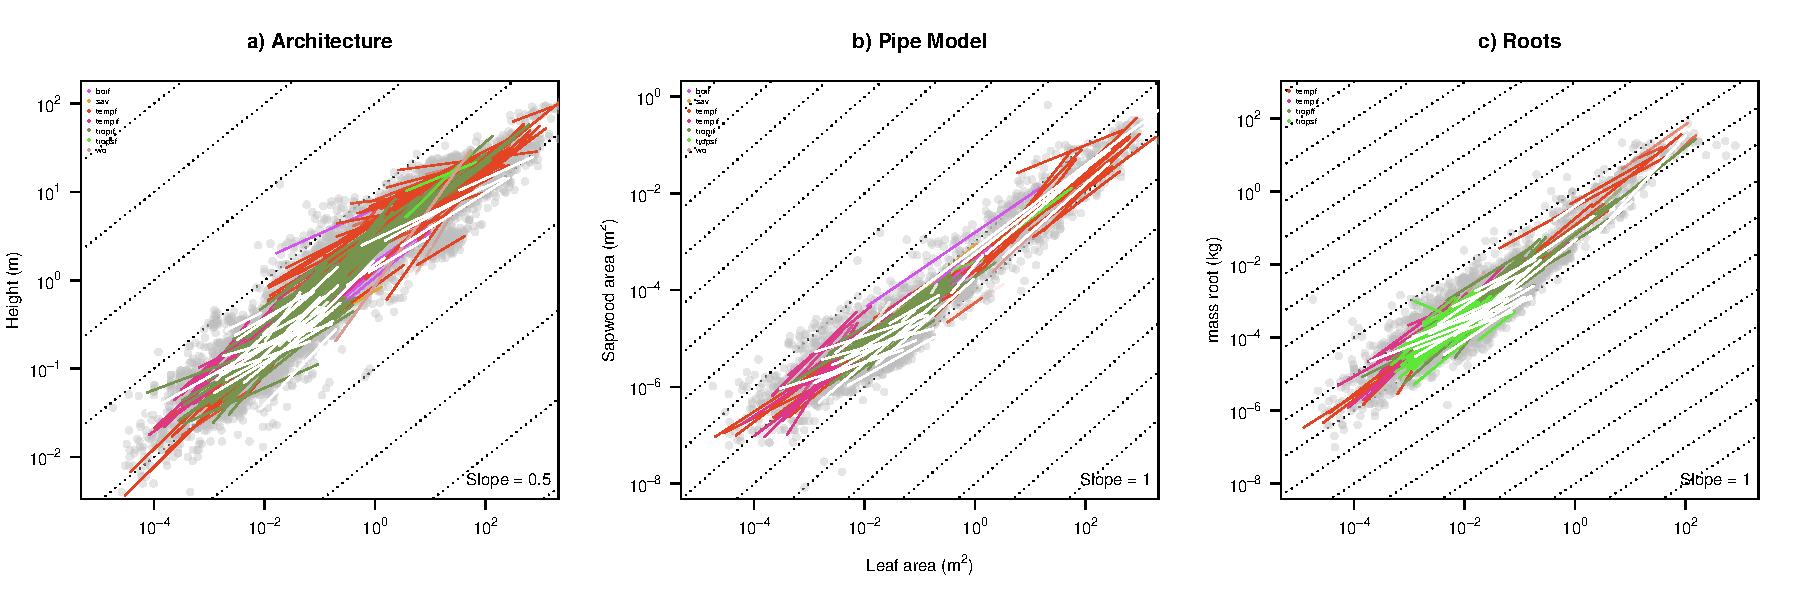
\includegraphics{main/allometry.pdf}
\caption{\textbf{Key assumptions of a functional balance and trait
trade-offs model, evaluated using global dataset.} We used the biomass and
allometry database to evaluate model assumptions about \textbf{a,}
scaling of leaf area with plant height, \textbf{b} Scaling of sapwood
area with leaf area, and \textbf{c} scaling of root mass with leaf area.
Each dot is a single plant. Lines show standardised major axis lines
fitted to data from each site, with intensity of shading adjusted
according to strength of the relationship. Colours indicate vegetation
type. Dashed black lines show values expected under functional-balance
assumption (see Supplementary text for details). \label{f-assumptions}}
\end{figure}

\newpage

\begin{figure}[ht]
\centering
\includegraphics{main/growth_light_dia.pdf}
\caption{\textbf{Traits moderate the responsiveness of growth to changes
in light environment (diameter growth).} Panels show predicted relationship between
specific trait and diameter growth rate, for a plant of specified
diameter and under a range of shading environments.
\label{f-growth_light_dia}}
\end{figure}

\begin{figure}[ht]
\centering
\includegraphics{main/growth_light_mass.pdf}
\caption{\textbf{Traits moderate the responsiveness of growth to changes
in light environment (mass growth).} Panels show predicted relationship between
specific trait and diameter growth rate, for a plant of specified
diameter and under a range of shading environments.
\label{f-growth_light_mass}}
\end{figure}

\newpage

\begin{figure}[ht]
\centering
\includegraphics{main/max_leaf_above.pdf}
\caption{\textbf{The effect of traits on growth changes with size and
light environment.} Traits moderate the responsiveness of growth to changes in light
environmentThis figure needs to show more of key result with respect to to size.
Possibly separate figure. \label{f-shifts}}
\end{figure}

\newpage

\begin{figure}[ht]
\centering
\includegraphics{main/max_leaf_above.pdf}
\caption{\textbf{Low construction cost leads to shade intolerance,
because of costs of high turnover.} Panels show effect of traits on
maximum amount of shading that can be endured before net production (eq.
\ref{eq:dbdt}) reaches zero. Lines indicate relationship for plants of a
given height. \label{f-wplcp}}
\end{figure}

\clearpage

\begin{appendices}
\setcounter{figure}{0} \renewcommand{\thefigure}{S\arabic{figure}}
\setcounter{table}{0} \renewcommand{\thetable}{S\arabic{table}}

\section{Relationship between traits and relative growth rate} \label{app:traits-RGR}

We start with eq. \ref{eq:dbdt} for mass-based growth. For seedlings, which are
young and mostly leaf, it is reasonable to ignore all turnover terms as
well as the respiration terms for non-leaf tissues. Net production then
becomes a linear function of leaf area and net photosynthesis per leaf
area ($A_\textrm{net} = y(A - r_{\rm l})$), making relative growth
rate a linear function of $\phi$:

\begin{equation}\label{eq:RGR}
\underbrace{\strut\frac{{\rm d}B}{{\rm d}t}\frac{1}{M_{\rm a}}}_\textrm{relative growth in mass}  \approx A_\textrm{net} \times \phi^{-1} \times \frac{M_{\rm l}}{M_{\rm a}}. \end{equation}

Although Eq. \ref{eq:RGR} captures patterns of growth in seedlings in
relation to $\phi$\citep{Wright-2000}, this
approximation does not directly link to other traits, or to the
variables that are routinely collected for large trees: namely plant
height ($h$) and stem cross-sectional area ($A_{\rm st}$) or
diameter $D$.


\section{Derivation of a simple allometric model of plant
function}\label{app:func_balance}

Here we describe an allometric model linking the various size dimensions
of a plant required by most ecologically realistic vegetation models
(i.e. =mass of leaves, mass of sapwood, mass of bark, mass of fine
roots) to a plant height. Table \ref{tab:allometry} provides a summary
of the derived model, while Table \ref{tab:params} provdies estimates on
key parameters.


\subsection{Leaf area}\label{leaf-area}

Based on empirically observed allometries (see main text), we assume an
allometric log-log scaling relationship between the accumulated leaf
area of a plant and its height:

\begin{equation}\label{eq:ha}
A_{\rm l}=\alpha_1 \, h^{\beta_1}.
\end{equation}

Note, scaling relationship reversed from \citep{Falster-2011}.

\subsection{Mass of sapwood}\label{mass-of-sapwood}

We follow the model of \citep{Yokozawa-1995} describing the
vertical distribution of leaf area within the crowns of individual
plants. This model can account for a variety of canopy profiles through
a single parameter $\eta$. Setting $\eta=1$ results in a conical
canopy, as seen in many conifers, while higher values, e.g. $\eta=12$
, give a top-weighted canopy profile similar to those seen among
angiosperms. Let $S(z,h)$ be the sapwood area at height $z$ for a
plant with top height $h$. Following Yokozawa and Hara (1995) we
assume a relationship between $S(z,h)$ and height such that

\begin{equation}\label{eq:crown1}
\frac{S(z,h)}{S(0,h)}= \big(1-\big(\frac{z}{h}\big)^\eta\big)^2.
\end{equation}

We also assume that each unit of sapwood area supports a fixed area of
leaf (the pipe model, \citep{Shinozaki-1964}), so that the total
canopy area of a plant relates to basal sapwood area $S(0,h)$:

\begin{equation}\label{eq:crown2}
\frac{M_{\rm l}}{\phi}= \theta \, S(0,h).
\end{equation}

Integrating $S(z,h)$ gives a solution for the total mass of sapwood in
the plant:

\begin{equation}\label{eq:ms1}
M_\textrm{s}=\rho \, \int_0^h \, S(z,h) \, {\rm d}z= \rho \, S(0,h) \, h \, \eta_c, \end{equation}

where
$\eta_c=1-\frac{2}{1+\eta} + \frac{1}{1+2\eta}$ \citep{Yokozawa-1995}.
Substituting from eq. \ref{eq:crown2} into eq. \ref{eq:ms1} gives an
expression for sapwood mass as a function leaf area and height:

\begin{equation}\label{eq:ms2}
M_\textrm{s}=\rho \, \eta_c \, \theta \, A_{\rm l} \, h.
\end{equation}

\subsection{Bark mass}\label{bark-mass}

Bark and phloem tissue are modelled using an analogue of the pipe model,
leading to a similar equation as that for sapwood mass (eq.
\ref{eq:ms2}). Cross sectional-area of bark per unit leaf area is
assumed to be a constant fraction $b$ of sapwood area per unit leaf
area such that

\begin{equation}\label{eq:mb}
M_{\rm b}=b M_\textrm{s}.
\end{equation}

\subsection{Root mass}\label{root-mass}

Also consistent with pipe-model assumption, we assume a fixed ratio of
root mass per unit leaf area

\begin{equation}\label{eq:mr}
M_{\rm r}=\alpha_3 \, A_{\rm l}.
\end{equation}

Even though nitrogen and water uptake are not modelled explicitly,
imposing a fixed ratio of root mass to leaf area ensures that
approximate costs of root production are included in calculations of
carbon budget.

\section{Effect of traits on height growth} \label{app:traits_max}

We want to show how two traits $\phi$ and $\rho$ influence growth rate,
by looking at the effect of
traits on the components of growth rate (eq. \ref{eq:dhdt}. To make
the analysis more tractable, we will assume we are dealing with a plant of
given height where 100\% of available energy is allocated to growth,
i.e. $\frac{{\rm d}M_{\rm a}}{{\rm d}B}=1$. Note also
that by the assumptions of our model and above, traits do not influence
$\frac{{\rm d}H} {{\rm d}A_{\rm l}}$. Thus we have

\begin{equation} \label{eq:G2}
G = \frac{{\rm d}H}{{\rm d}t} = c_1   \left(\frac{{\rm d}A_{\rm l}} {{\rm d}M_{\rm a}}  \frac{ {\rm d}B} {{\rm d}t} \right),
\end{equation}

where $c_1 = \frac{{\rm d}H}{{\rm d}A_{\rm l}}$. Eq.
\ref{eq:G2} is a product of the form $Y(x) = W(x) \times Z(x)$. For,
equations of this type, the derivative $\partial{Y}/\partial{x}$ is
given by $\partial{W}/\partial{x} \, Z + W \, \partial{Z}/\partial{x}$. Thus
the derivative of $G$ with respect to some trait $x$  is given by

\begin{equation} \label{eq:dG}
\frac{\partial G} {\partial x} =
\frac{\partial \left(\frac{{\rm d}A_{\rm l}} {{\rm d}M_{\rm a}}\right)}{\partial x}
 \, \frac{ {\rm d}B} {{\rm d}t}
+ \frac{{\rm d}A_{\rm l}} {{\rm d}M_{\rm a}}
\, \frac{\partial \left( \frac{ {\rm d}B} {{\rm d}t}\right)}{\partial x}.
\end{equation}

If this derivative is positive (negative), there will be a positive (negative) relationship
between traits and growth at the height where it is evaluated.

We further simplify by expanding the derivative of eq. \ref{eq:daldmt}:

\begin{equation} \label{eq:dA_dx}
\frac{\partial \left(\frac{{\rm d}A_{\rm l}} {{\rm d}M_{\rm a}}\right)}
{\partial x} = -\left(\frac{{\rm d}A_{\rm l}} {{\rm d}M_{\rm a}}\ \right)^2
\, \frac{\partial \left(\frac{{\rm d}M_{\rm a}} {{\rm d}A_{\rm l}}\right)
}{\partial x}.
\end{equation}

Combing eqs. \ref{eq:dG}-\ref{eq:dA_dx}, we have

\begin{equation} \label{eq:dG2}
\frac{\partial G} {\partial x} =
\frac{{\rm d}A_{\rm l}} {{\rm d}M_{\rm a}}
\left(
\frac{\partial \left( \frac{ {\rm d}B} {{\rm d}t}\right)}{\partial x}
- \frac{{\rm d}A_{\rm l}} {{\rm d}M_{\rm a}}
\,  \frac{\partial \left(\frac{{\rm d}M_{\rm a}} {{\rm d}A_{\rm l}}\right)
}{\partial x}
 \, \frac{ {\rm d}B} {{\rm d}t}
\right).
\end{equation}

Since is $\frac{{\rm d}A_{\rm l}} {{\rm d}M_{\rm a}}>0$ always, the sign
of $\frac{\partial G} {\partial x}$ depends on the terms inside the brackets on the
RHS. Rearranging we find that $\frac
{\partial G} {\partial x} < 0$ if

\begin{equation}\label{eq:dg3}
\frac{\partial \left( \frac{ {\rm d}B} {{\rm d}t}\right)}{\partial x}
< \frac{{\rm d}A_{\rm l}} {{\rm d}M_{\rm a}}
\,  \frac{\partial \left(\frac{{\rm d}M_{\rm a}} {{\rm d}A_{\rm l}}\right)
}{\partial x} \, \frac{ {\rm d}B} {{\rm d}t},
\end{equation}

or equivalently
\begin{equation}\label{eq:dg4}
\frac{
\frac{\partial \left( \frac{ {\rm d}B} {{\rm d}t}\right)}{\partial x} }
{\frac{ {\rm d}B} {{\rm d}t}}
<
\frac{ \frac{\partial \left(\frac{{\rm d}M_{\rm a}} {{\rm d}A_{\rm l}}\right)
}{\partial x}}{\frac{{\rm d}M_{\rm a}} {{\rm d}A_{\rm l}}}.
\end{equation}

In words, there will be a negative relationship between trait x and growth if the
relative change in production due to change in traits is less than the relative change
in the total construction cost for a unit of leaf area due to change in trait. Crucially,
key elements in eq. \ref{eq:dg3} are modified by height.

We can also solve for trait values $x$ maximising growth rate, i.e. the value
giving $\partial G /\partial x = 0$:

\begin{equation}\label{eq:max}
\frac{
\frac{\partial \left( \frac{ {\rm d}B} {{\rm d}t}\right)}{\partial x} }
{\frac{ {\rm d}B} {{\rm d}t}}
=
\frac{ \frac{\partial \left(\frac{{\rm d}M_{\rm a}} {{\rm d}A_{\rm l}}\right)
}{\partial x}}{\frac{{\rm d}M_{\rm a}} {{\rm d}A_{\rm l}}}.
\end{equation}

\subsection{Leaf construction cost}

If the trait of interest is leaf-construction cost, i.e. $x=\phi$, we can expand
eq. \ref{eq:dg4} as follows. Note that $\frac{\partial \left(\frac{{\rm d}M_\textrm
{t}} {{\rm d}A_{\rm l}}\right)}{\partial \phi} = 1$. Also, from eq. \ref{eq:dbdt} we obtain,

\begin{equation}\label{eq:dbdt2}
\frac{{\rm d}B}{{\rm d}t} = c_2 - A_{\rm l} A_4 \phi ^{1-B_4}
\end{equation}

where
$c_2 = y ( A_{\rm l} \, (A - r_{\rm l}) + \sum_\textrm{i=b,s,r}{M_\textrm{i} \, r_\textrm{i}}) - (\sum_\textrm{i=b,s,r}{M_\textrm{i} \, hmax\textrm{i}})$
is independent of $\phi$, and thus

\begin{equation}\label{eq:dbdt3}
\frac{\partial \left( \frac{ {\rm d}B} {{\rm d}t}\right)}{\partial \phi}  =
(B_4-1) A_{\rm l} A_4\phi ^{-B_4}.
\end{equation}

Eq. \ref{eq:dbdt3} shows that if $B4=1$, $\frac{ {\rm d}B} {{\rm d}t}$ is independent
of $\phi$. In contrast, if $B4>1$ (which tends to be the case empirically), $\frac{ \textrm
{d}P} {{\rm d}t}$ increases as $\phi$ increases, more acutely at low $\phi$.

Substituting into eq. \ref{eq:dg4}, we have the result that growth rate correlates
with traits if

\begin{equation} \label{eq:G6}
\frac{(B_4-1) A_{\rm l} A_4\phi ^{-B_4}}{c_2 - A_{\rm l} A_4 \phi ^{1-B_4}}
< \frac{1}{\phi
 + \frac{{\rm d}M_\textrm{s}}{{\rm d}A_{\rm l}} + \frac{{\rm d}M_\textrm
 {b}}{{\rm d}A_{\rm l}} + \frac{{\rm d}M_{\rm r}}{{\rm d}A_{\rm l}}}.
\end{equation}

\subsection{Wood construction cost}

Do similar to previous section for wood construction cost.

\newpage

\section{Supplementary tables}\label{supplementary-tables}

\begin{table}[ht]
\caption{Model parameters}
\centering
{\footnotesize  % smaller font, double space
\begin{doublespace}
% \include{table-pars}

\end{doublespace}
}
\label{tab:params}
\end{table}

\newpage

\section{Supplementary figures}\label{supplementary-figures}

\begin{figure}[ht]
\centering
\includegraphics{SI/lmA_tradeoff.pdf}
\caption{\textbf{Leaf turnover decreases with leaf-construction cost.}
Data from \citep{Wright-2004} for 678 species from 51 sites, each
point giving a species-average. Lines show standardised major axis lines
fitted to data from each site, with intensity of shading adjusted
according to strength of the relationship.\label{fS-leaf}}
\end{figure}


\newpage

\begin{figure}[ht]
\centering
\includegraphics{SI/mass_fraction.pdf}
\caption{\textbf{Change in allocation with size.}
\label{f-mass_fraction}}
\end{figure}

\newpage

\begin{figure}[ht]
\centering
\includegraphics{SI/lmA_effects_at_diameters.pdf}
\caption{\textbf{The expected correlation between leaf-construction cost
and growth rate changes with plant size.} \label{f-lmA_growth_size}}
\end{figure}

\begin{figure}[ht]
\centering
\includegraphics{SI/lmA_effects_at_diameters_relative.pdf}
\caption{\textbf{The expected correlation between leaf-construction cost
and relative growth rate changes with plant size.}
\label{f-lmA_growth_size_relative}}
\end{figure}

\begin{figure}[ht]
\centering
\includegraphics{SI/rho_effects_at_diameters.pdf}
\caption{\textbf{The expected correlation between stem-construction cost
and growth rate changes with plant size.} \label{f-rho_growth_size}}
\end{figure}

\begin{figure}[ht]
\centering
\includegraphics{SI/rho_effects_at_diameters_relative.pdf}
\caption{\textbf{The expected correlation between stem-construction cost
and relative growth rate changes with plant size.}
\label{f-rho_growth_size_relative}}
\end{figure}

\begin{figure}[ht]
\centering
\includegraphics{SI/hmat_effects_at_diameters.pdf}
\caption{\textbf{The expected correlation between maximum height and
growth rate changes with plant size.} \label{f-hmat_growth_size}}
\end{figure}

\begin{figure}[ht]
\centering
\includegraphics{SI/hmat_effects_at_diameters_relative.pdf}
\caption{\textbf{The expected correlation between maximum height and
relative growth rate changes with plant size.}
\label{f-hmat_growth_size_relative}}
\end{figure}


\end{appendices}
\end{document}